\documentclass{article}
\usepackage[utf8]{inputenc}
\usepackage{graphicx} %Used for graphics processing and scaling
% \usepackage{geometry}
\usepackage{multicol} %Add the multicolumn feature used for two-column names
% \usepackage[sfdefault]{josefin} %Change of Font
\usepackage{xcolor} %Allows for the naming colors using their rgb values
\usepackage[hidelinks]{hyperref} %Allows hyperlinking of table of contents and references
%The `hidelinks` options remove the ugly border lines across references
\usepackage{enumitem} %Allows for the use of `noitemsep` in itemize environments
\usepackage{listings} %Allows the typesetting of programming codes so that they will appear properly as codes

%Defining of colors as names so that we can use their names rather than their RGB values each time we refer to them
\definecolor{codegreen}{rgb}{0,0.6,0}
\definecolor{codegray}{rgb}{0.5,0.5,0.5}
\definecolor{codepurple}{rgb}{0.58,0,0.82}
\definecolor{backcolour}{rgb}{0.95,0.95,0.92}

\lstdefinestyle{mystyle}{ %Default style of the typesetting of code is ugly, so this style is created (not yet used)
    backgroundcolor=\color{backcolour},
    commentstyle=\color{codegreen},
    keywordstyle=\color{magenta},
    numberstyle=\tiny\color{codegray},
    stringstyle=\color{codepurple},
    basicstyle=\ttfamily\footnotesize,
    breakatwhitespace=false,
    breaklines=true,
    captionpos=b,
    keepspaces=true,
    numbers=left,
    numbersep=5pt,
    showspaces=false,
    showstringspaces=false,
    showtabs=false,
    tabsize=2
}

\lstset{style=mystyle} %This activates the created style. Note that this is the default activation. You can multiple styles and use different style of each block of code


\usepackage[style=apa]{biblatex} %Package used to enable referencing
\addbibresource{Diola-Mondido---Final-Project-References---CMSC_124.bib} %Bibliography file



\begin{document}

% \maketitle

\thispagestyle{empty}

\begin{center}
    \begin{figure}
        \centering
        
\includegraphics[scale=0.5]{UP-Cebu-Logo}
        % \caption{Caption}
        % \label{fig:title_page_logo}
    \end{figure}

    \textbf{University of the Philippines Cebu}\\
    College of Science\\
    Department of Computer Science\\
    \par
    \bigskip
    Design and Implementation of Programming Languages\\
    (CMSC 124)

\rule{\textwidth}{0.4pt}
\vfill

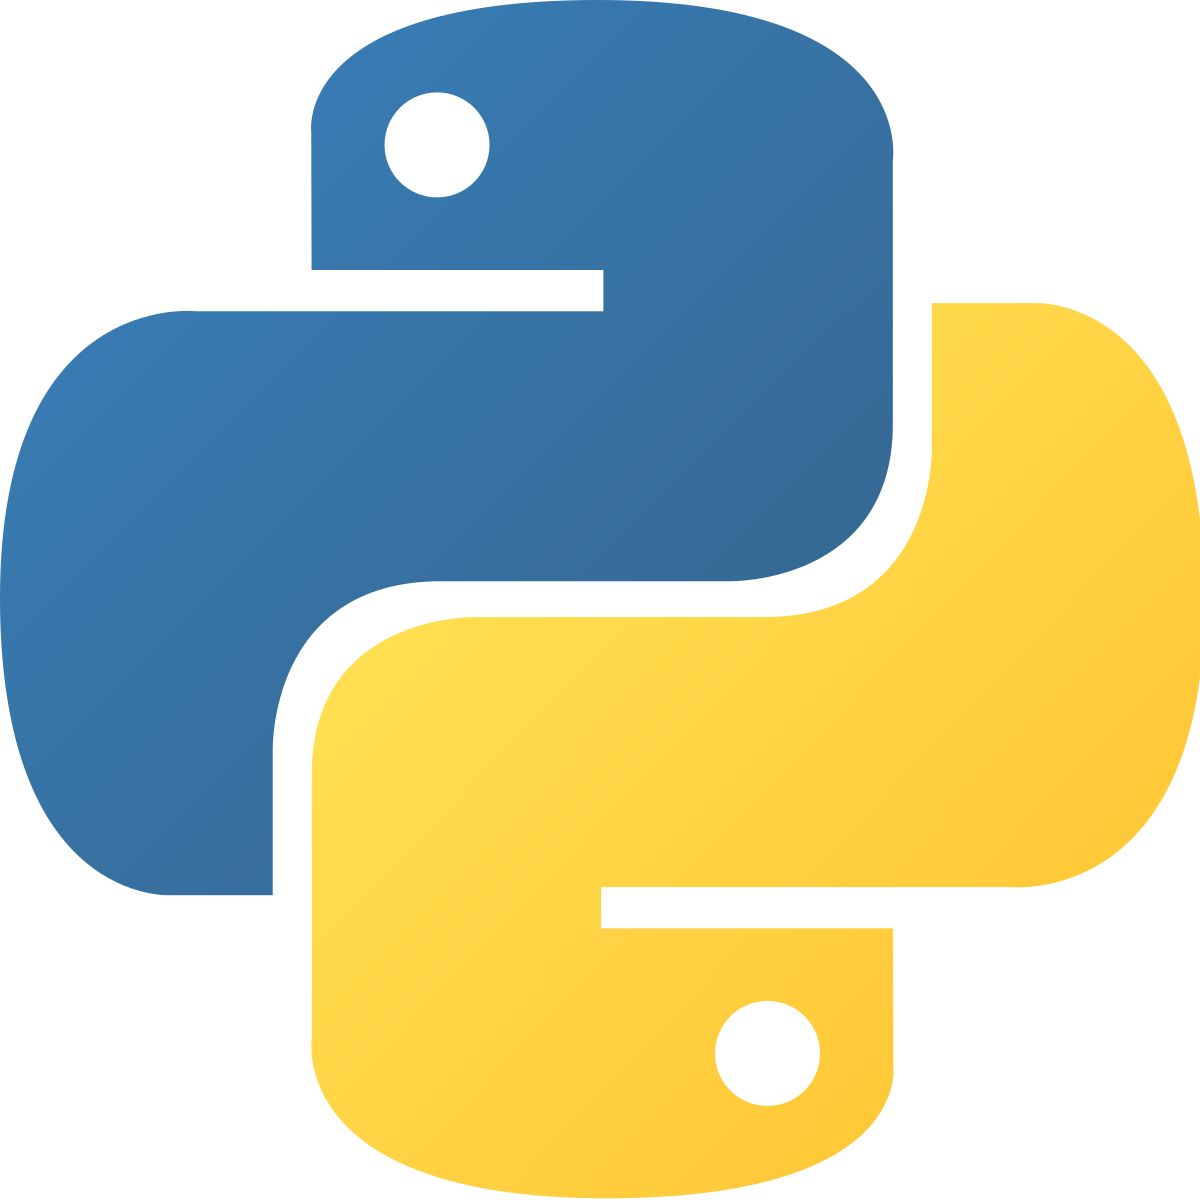
\includegraphics[scale=0.05]{Python-Logo.png}\qquad
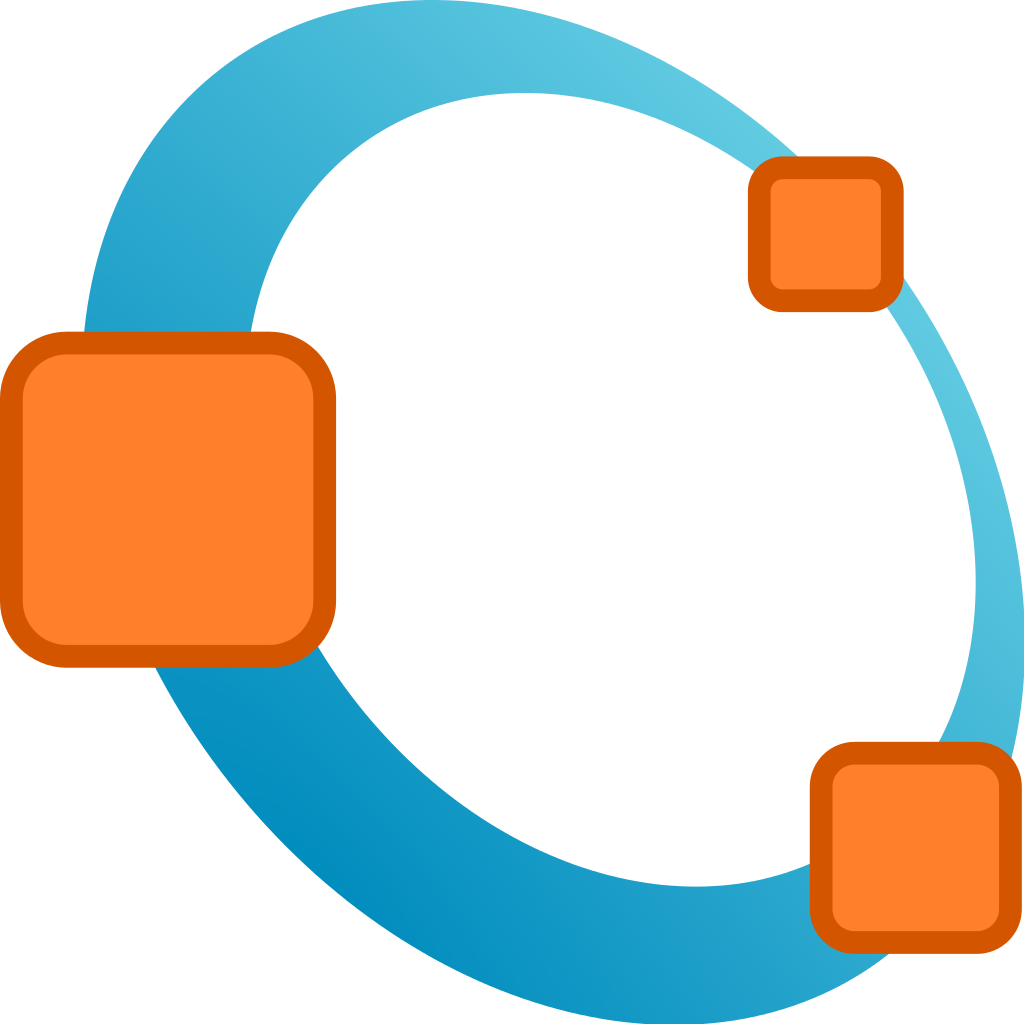
\includegraphics[scale=0.06]{GNU-Octave-Logo.png}\\
\bigskip
\textbf{\large Python and Octave:\\Characteristics and Comparison}\\
\medskip Final Project

\vfill

\rule{\textwidth}{0.4pt}
\vfill
\begin{multicols}{2}

\begin{center}
    \textbf{Alex A. Diola}\\
    2019-11984\\
    \href{mailto:aadiola@up.edu.ph}{aadiola@up.edu.ph}\\
    CMSC 124-B\\
\end{center}

\columnbreak

\begin{center}
    \textbf{Dianne M. Mondido}\\
    2019-04460\\
    \href{mailto:dmmondido2@up.edu.ph}{dmmondido2@up.edu.ph}\\
    CMSC 124-B\\
\end{center}
\end{multicols}


\vfill

\par
\textit{1st semester}\\
\textit{2021-2022}
\end{center}

\pagebreak

\renewcommand{\contentsname}{Table of Contents} %Change table of contents label from "Contents" to "Table of Contents"
\tableofcontents

\setlength{\parskip}{1em} %Increase distance between paragraphs

\pagebreak

\addcontentsline{toc}{section}{\LaTeX\ source code file}
\section*{\LaTeX\ source code file}


The \LaTeX\ source code file can be found \href{https://www.overleaf.com/read/pqfsqzyzffhp}{here}:\\
\texttt{https://www.overleaf.com/read/pqfsqzyzffhp}.\\This link, however, only gives read access as the tool used (OverLeaf) only allows for a maximum of two (2) collaborators (read-write access) in its free version, and these two are already used by the authors of the paper.




\pagebreak

\addcontentsline{toc}{section}{Python}
\section*{Python}

\addcontentsline{toc}{subsection}{Purpose and Motivation}
\subsection*{Purpose and Motivation}
\par
Python is an interpreted high-level programming language that emphasizes simplicity and efficiency in its philosophy. Like any other programming language, Python has plenty of applications for almost all fields such as:
\begin{itemize}[noitemsep]
\item Data Science
\item Scientific and mathematical computing
\item Web development
\item Finance and trading
\item System automation and administration
\item Computer graphics
\item Basic game development
\item Security and penetration testing
\item General and application-specific scripting
\item Mapping and geography (GIS software)
\end{itemize}
\par
Python was created with simplicity as its goal. That is why it is considered an important programming language to learn as it is commonly used in the industry. According to TIOBE index, Python is ranked 1st as the highest increase rating of 2021 and still ranked first in January of 2022. In addition, it is also the most searched Programming Language (PL) tutorial.
\par
Python was created because the existing programming languages during that time were time-consuming to learn and hard to understand. With these limitations, Python was created.

\addcontentsline{toc}{subsection}{History}
\subsection*{History}
\par
On February 20, 1991, Dutch Programmer Guido Van Rossum first released his invention, Python, which actually came from an old BBC television comedy sketch series named Monty Python’s Flying Circus.
\par
Before Python came to be, Guido Van Rossum used to work at CWI working for a distributed system called Amoeba. C was the used language at his work, yet he felt that the language was too time-consuming. Therefore, he began developing a new language that supports simplicity and efficiency in his free time. What makes Python interesting is the unique mixture of C bash script capabilities and again, its simplicity. Guido Van Rossum heavily relied on the ABC programming language but also included tools for imperative programming and dynamic types.
\par
Unlike other programming languages that rely heavily on professionals and large companies to develop features of that language, Python continuously spread and evolved around the world with the contributions from anonymous programmers, users, testers, and enthusiasts in which most of them are not IT specialists. Through Van Rossum’s idea and continuous effort of the community, Python became the most used programming language across the world.

\addcontentsline{toc}{subsubsection}{Development of Python}
\subsubsection*{Development of Python}
\par
Guido Van Rossum published the first open-source version (Python version 0.9.0) at alt.sources. This version already includes functions, exception handling, and the core data types of list, dict, str, and others. Moreover, it had already supported object-oriented programming and had a module system.

\par
\noindent
\textit{Python 1}

\par
Python’s next version (Python version 1.0) was released in January 1994. The major features of this version now supported functional programming tools such as map, filter and reduce, and lambda. In version 1.4, it brought the Modula–3 style keyword arguments and support for complex number operations.

\par
\noindent
\textit{Python 2}

\par
Python 2.0 was launched in 2000 with a huge change in its source code. It now supports many desired features such as:
\begin{enumerate}

    \item Unicode\\
    The Unicode string data type now allocates 16-bit numbers to represent characters instead of the 8-bit strings. This means that there are an additional 65,000 supported symbols from non-Latin script languages like Russian, Chinese, or Arabic to non-letter characters like emojis.

    \item List Comprehension\\
    These are used to create lists from different iterables. It takes and returns a list, allowing the user to trim to a specific need or to create a new list with newly manipulated elements.

    \item Garbage Collection\\
    Python now switches its garbage collection cycles from counter-based system to cycle-based systems. In the counter-based system, each object contains a counter that records how many other objects are pointing to it. In deleting, the objects are automatically deleted when the counter reaches zero. The disadvantage of using this system is that it couldn’t delete objects that were pointed to but were not accessible, resulting in a memory leak. The cycle-based system fixes that problem by using periodic cycles to call the garbage collector to delete inaccessible objects. The cycles use additional overhead but reduce the risk of a memory leak. Overhead costs of the deletion cycles have since been reduced due to optimizations.

    \item Assignment Shortcutes\\
    This version fully supports a shorter version of assigning variables. The list of supported assignment operators include \verb|+=|, \verb|-=|, \verb|*=|, \verb|/=|, \verb|%=|, \verb|**=|, \verb|&=|, \verb!|=!, \verb|^=|, \verb|>>=|, and \verb|<<=|. These operators are important for simplicity and readability of the code.

    \item Other Improvements\\
    Although Python 2 terminated its support in June of 2009, there are still some functions they added. Support for nested scopes was added to perform like other statically scoped languages. Generator routines for controlling loop behavior and creating unified types and classes into one Python hierarchy were added for a more object-oriented programming feel. Furthermore, here are some additions to the Python functionality:
    \begin{itemize}
        \item generator expressions for function decorators, decimal data types, and iterator function
        \item Added \texttt{with} statement and also its optimization
        \item Backwards compatible 1.0 features such as \texttt{bin()}, \texttt{typeError}, and \verb|_complex_()|.
    \end{itemize}

\end{enumerate}

\par
\noindent
\textit{Python 3}

\par
The rise of Python as a frontrunner for data science has been made possible by the big changes in Python 3. The aim of this update is to remove design flaws by deleting duplicated modules and constructs. This also means that Python 2 is not compatible with Python 3. In case the user wants to change its code from Python 2 to Python 3, there is a tool named 2to3 that will review and convert the syntax to Python 3 automatically. Listed below are the upgrades of Python 3:

\begin{enumerate}

    \item Print Built-in Function\\
    In Python 2, the \texttt{print} function needed to be imported from the \verb|__future__| module. Now, it is considered as a built-in function with arguments enclosed in parentheses.

    \item NumPy Library\\
    With the need of data automation tools, the NumPy library became a field for data enthusiasts. It became the preferred language for data science and machine learning followed by R, and MATLAB.

    \item Renaming raw-input to input\\
    Input now always returns a string rather than an expression. This is to remove confusion with two similar inputs and instead favor the more common use. Using \texttt{eval(input())} will let the user use the old functionality.

    \item Unification of \texttt{str} and unicode\\
    All text content such as strings is now Unicode by default. This is to reduce errors caused by mixing Unicode and encoded data types of the same program. If the user opts for encoded string, the user can use an immutable bytes type by using the method \texttt{bytes()} or a mutable bytes type through \texttt{bytearray()} method. The advantage of using bytes is that they can store varying data whereas Unicode only represents text-like data.

    \item Integer Division\\
    Division operations now return an int data type instead of float. This is to remove unexpected behavior from unintentional truncation \parencite{thelin_2021}.

    \item Support for asynchronous programming\\
    With the use of an async module, it can now handle event loop implementations, coroutines, asynchronous iteration and context managers, and awaitable objects. The reserved keywords \texttt{async} and await, and the method \texttt{breakpoint()} were added to the module.

    \item Other improvements\\
    Although Python 2 is incompatible with Python 3, reusing functions is still common when updating versions of the programming languages. Some changes in exception handling was implemented such as the need for the keyword as (e.g. exec as *var*). The \texttt{with} statement is now built-in like \texttt{print} function. Renaming some methods were also implemented for readability, simplicity, and writability.

\end{enumerate}

\addcontentsline{toc}{subsection}{Features}
\subsection*{Features}
\par
Python is an interpreted, free-source, object-oriented, high-level programming language with dynamic semantics (Python). From the definition itself, Python has several features that fit the needs of almost all users and fields. With its continuous support and contributions from the community, Python has yet to plummet its popularity. Here are some features of Python:

\begin{enumerate}

    \item Easy to use\\
    High-level languages tend to become more human-readable than machine ones, but some of these languages aren’t easy for some beginners such as Java, C++, and C. Python’s philosophies are revolved around simplicity both in coding and reading that is why Python is the most searched language for it is easy to use and learn.

    \item Free-Open Source\\
    Python is made available to the public through its website with support from different operating systems and without the need for financial subscriptions or contributions.

    \item Object-oriented Programming\\
    Python supports OOP concepts such as encapsulation, classes, polymorphism, inheritance, etc. This paradigm helps users to reuse code for efficiency. Python caters to a lot of programming paradigms such as procedural, functional, declarative, and more.

    \item Interpreters than compilers\\
    Python translates programs one line at a time compared to compilers that scan the entire line first and then translate them to machine code. Interpreters help to debug efficiently both in time and memory.

    \item Large Standard Libraries\\
    For Python to be applicable to most of the different fields with their needs, a vast library should be able to help them find the solutions to their problem. There are standard libraries good for data science, web development, machine learning, and even scripting. Libraries such as NumPy, TensorFlow, Pandas, Django, Pytorch, and more are some of the most used libraries in Python for different projects in different fields.

    \item Supports GUI Programming\\
    With its vast libraries, Python can also be used for graphics interfaces. PyQT5, Tkinter, Kivy are the libraries that are used for developing web applications.

    \item Integratable to other Programming Languages\\
    Python can also be integrated through different programming languages such as C, C++, Java, and more. This is one of the advantages of having interpreters

    \item Dynamic Memory Allocation\\
    Specifying data types is no longer needed when coding in Python since it automatically allocates the memory to the variable at run time. This means that a variable’s data type is decided at run-time, not in advance.

\end{enumerate}


\addcontentsline{toc}{subsection}{Paradigms}
\subsection*{Paradigms}
\par
Most modern programming languages have a philosophy for multi-paradigm programming since different users have different needs. Developers must be able to meet their demands now that innovations are constantly improving.
\par
Python is considered a multi-paradigm programming language. Here are some paradigms that Python supports.

\par
\noindent
\textit{Object-Oriented Paradigm}

\par
The key feature of object-oriented programming is the “object” styled way of thinking. An object is termed as the instance of a class that consists of data members and methods. This programming paradigm supports classes, encapsulation, abstraction, and inheritance that will make coding more efficient.

\par
\noindent
\textit{Procedural Paradigm}

\par
In procedural programming, a series of computations and procedures in the program are executed in a systematic order of statements, functions, and commands to complete a computational program. This programming paradigm facilitates the practice of good program design, organization due to its container-style programming, and modularization.

\par
\noindent
\textit{Functional Paradigm}

\par
Python also supports the functional programming paradigm because it can bind pure mathematical functions and manages every statement as functional expressions and declarations rather than the execution of statements. Recursion and Lambda expression are one of the approaches of functional programming. This programming paradigm focuses more on “what to solve” than “how to solve” like in procedural programming.

\addcontentsline{toc}{subsection}{Language Evaluation}
\subsection*{Language Evaluation}

\addcontentsline{toc}{subsubsection}{Readability}
\subsubsection*{Readability}
\par
Python is fairly easy to read and understand by people with or without much experience in programming using this language and is the easiest to read among the languages compared here. Since its philosophy emphasizes more on simplicity and readability, its use of fewer yet readable constructs is a feature that highlights orthogonality. In addition, Python is the closest to the natural language, English, than other PLs whose syntax design is closest to machine code. Python has well-defined control and extensive data structures since its memory is dynamically allocated so users don't need to define the data type. Although, this lack of explicit data typing may somehow be a disadvantage when code reviewing.

\addcontentsline{toc}{subsubsection}{Writability}
\subsubsection*{Writability}
\par
As Python is easy to read, it also has good writability. Python is very easy to write since it has simple constructs and dynamic memory allocation. Users can still write a simple program to complex ones with efficiency in writing them since it uses fewer constructs. This also means that expressivity exists in Python because there is more work done in a single line of code than a single line of code in other languages. Although, expressivity may sometimes confuse users like using the operator \texttt{==}, \texttt{===}, and \texttt{is}.

\addcontentsline{toc}{subsubsection}{Reliability}
\subsubsection*{Reliability}
\par
Python’s exception handling and aliasing features are quite reliable. In aliasing,  variables in Python are just containers that store references to values. Though there is no type checking, the intuitive syntax as well as the extensive exception handling capabilities and runtime debugging greatly make up for this.

\addcontentsline{toc}{section}{Octave}
\section*{Octave}

\addcontentsline{toc}{subsection}{Purpose and Motivation}
\subsection*{Purpose and Motivation}
\par
GNU Octave is a high-level programming language that consists of a powerful mathematics-oriented syntax that supports 2D and 3D plotting and visualization tools. It provides a command-line interface for solving linear and nonlinear problems numerically, and for performing other numerical-based problems using a language compatible with MATLAB (GNU).
\par
It provides extensive tools for solving mathematical problems such as linear algebra problems, finding the roots of nonlinear equations, integrating ordinary functions, manipulating polynomials, and integrating ordinary differential and differential-algebraic equations. It can be extended and customized further by creating user-defined functions written in Octave itself, or by using dynamic libraries written in C, C++, Fortran, or other languages.
\par
It is easily extensible and customizable via user-defined functions written in Octave’s own language, or using dynamically loaded modules written in C++, C, Fortran, or other languages.
\par
Octave was created to be a companion for a chemical reactor design textbook for a chemical engineering course but throughout its development, it became a general flexible tool that is used widely in fields other than chemical engineering. Nowadays, it is used for teaching, research, and commercial applications.


\addcontentsline{toc}{subsection}{History}
\subsection*{History}
\par
Octave was originally conceived around 1988 to be an accompanying software for a chemical reactor design textbook authored by James Rawlings of the University of the Wisconsin-Madison and John Ekerdt of the University of Texas. It was initially intended to be specialized in solving chemical reactor design problems. However, this initial approach limited the capabilities of the tool being developed, and so the creators attempted to build a more flexible tool.
\par
During this time, Fortran was still very popular which is why people still opted for it as it is the computer language of engineering. However, the creators found that every time they tried to utilize Fortran, their students spent too much time debugging their Fortran code and not enough time was allotted to learning about chemical engineering. The creators believed that in a more interactive environment, such as the case for Octave, most students would be able to grasp the basics easily and use the tool with ease in just a few hours.
\par
In the Spring of 1992, the creators began the full-time development of Octave. The first alpha version of Octave was released on January 4, 1993. More than a year later, version 1.0 was released on February 17, 1994. Octave has undergone several major revisions. It is also included in several GNU/Linux distributions.
\par
When talking about Octave, people typically think about a musical note. However, the GNU Octave is from the name of the creator’s former professor, Prof. Octave Levenspiel. Professor Octave wrote a popular textbook on chemical reaction engineering and is known for its ability to do quick back-of-the-envelope calculations.

\addcontentsline{toc}{subsubsection}{Development of Octave}
\subsubsection*{Development of Octave}
\par
The latest stable release (as of writing) of Octave is version 6.4 It is worth noting that the creators somehow followed an unusual numbering scheme. For example, the first version after the alpha release was version 6.0 rather than the usual version 1.0. On this end, discussed below are the major revisions only. Major features not discussed below were introduced to Octave in iteration through minor revisions which are not included below but can found \href{https://wiki.octave.org/Release_History}{here}.

\par
\noindent
\textit{Version 1.1.0}

\par
Octave 1.1.0 was released on January 12, 1995. It has major updates when compared to the update to version 1.0 from 0.x.x.
\begin{enumerate}

    \item \texttt{Data structure} type (\texttt{struct} type)\\
    Added a new fundamental type in Octave which allows variables to act similar to C’s struct construct. This allows variables to hold sub-elements, e.g., \texttt{someVar.someUnderlyingAttribute = 124}.

    \item Exception Handling\\
    Octave now supports a limited form of exception handling modeled after the unwind-protect form of Lisp. This is useful to protect temporary changes to global variables from possible errors.

    \item Short-circuit evaluation\\
    The \verb|&&| and \verb!||! logical operators are now evaluated in a short-circuit fashion and work differently than the element by element operators \verb|&| and \verb!|!.

    \item Variable return list\\
    Octave can now return a list of values with unknown cardinality from functions. This means that it is no longer necessary to place an upper bound on the number of outputs that a function can produce.

    \item New functions and other improvements\\
    New functions for operating on polynomials have been added such as evaluation of polynomials at a point, deriving polynomials, integrating polynomials and others. Set manipulation and image processing functions have also been added.

\end{enumerate}

\par
\noindent
\textit{Version 2.0}

\par
Octave 2.0 was released on December 10, 1996.
\begin{enumerate}

    \item Crash handling\\
    If Octave crashes, it now attempts to save all user-defined variables in a file named \texttt{octave-core} in the current directory before exiting. This is very useful for processing intensive computations in which results take time to be computed.

    \item Ported to Windows\\
    Octave has been mostly ported to Windows NT and Windows 95 using the beta 17 release of the Cygnus GNU-WIN32 tools. While not all features work, it is already usable.

    \item User-defined data types\\
    A user can now add custom data-types by writing a class in C++. On systems that support dynamic linking, new data types can be added to an already running Octave binary.

    \item Improved exception handling\\
    A real exception-handling has been implemented using the try-catch method. In this case, the \texttt{catch} block is only implemented if there is an error caught in the \texttt{try} block.

    \item More functions and other improvements\\
    Several changes have been made to be compatible with newer versions of MATLAB. New functions have also been added for audio processing, file management, and others.

\end{enumerate}

\par
\noindent
\textit{Version 3.8}

\par
Octave 3.8 was released on December 27, 2013.
\begin{enumerate}

    \item Graphical User Interface\\
    While the new graphical user interface is not yet the default option when running Octave interactively, it is already working. As one of the most requested features throughout the years, it is one of the biggest updates in this version.

    \item Nested functions\\
    Octave now supports functions defined with other functions. The rules and scope of the nested functions are consistent with those used in Matlab.

    \item Named Exceptions\\
    Octave now has limited support for named exceptions. This is very useful for catching unique errors as well as easier debugging.

    \item \TeX{} Parser\\
    A \TeX{} parser has been implemented for the FLTK toolkit and is the default for any text object including titles and axis labels. Commands such \verb|\bf|, \verb|\it|, \verb|\rm|, etc. are now supported.

    \item Citation command\\
    This command returns the citation of Octave and used packages that the user can use in their papers and publications.

    \item More functions and other improvements\\
    Graphics processor has been changed to improved plotting and other visualization tools. New functions have also been added while outdated functions are deprecated or revised.

\end{enumerate}

\par
\noindent
\textit{Version 4.4}

\par
Octave 4.4 was released on April 30, 2018.
\begin{enumerate}

    \item Graphical Variable Editor\\
    It uses a spreadsheet-like interface for quick, intuitive editing of variables. This allows the user to easily edit variable values as well as view their real-time.

    \item Hash data structure\\
    A map data structure that allows efficient searching values using a key. This allows the user to efficiently store sets of data where the order is not important.

    \item More functions and other improvements\\
    External dependencies have been adjusted to accommodate newer versions of these external tools.

\end{enumerate}

\par
\noindent
\textit{Version 5.1}

\par
Octave 5.1 was released on February 23, 2019.
\begin{enumerate}

    \item High-Resolution support\\
    The Octave plotting system now supports high-resolution screens, i.e., those with greater than 96 DPI. This is useful for sharper details in visualization tools.

    \item Unicode support\\
    Support for Unicode characters in the names of files and folders accessed externally in Windows.

    \item More functions and other improvements\\
    External dependencies have been adjusted to accommodate newer versions of these external tools.

\end{enumerate}

\par
\noindent
\textit{Version 6.1}

\par
Octave 6.1 was released on November 26, 2020.
\begin{enumerate}

    \item Complex web service support\\
    Complex RESTful web services can now be accessed by the webread and webwrite functions. One major feature is the support for cookies to enable RESTful communication with the web service. This is really useful as the web continues to be the primary platform nowadays.

    \item More functions and other improvements\\
    External dependencies have been adjusted to accommodate newer versions of these external tools.

\end{enumerate}

\addcontentsline{toc}{subsection}{Features}
\subsection*{Features}
\par
Octave is an interpreted, free source, high-level programming language. From its conception, Octave was intended for numerical and math-related applications. Hence, it has several notable features that allow it to be used in teaching, research, and even commercial applications.
\begin{enumerate}
    \item Easy-to-use\\
    Octave was created to allow students to learn it easily and focus more on problems being solved than the language being used. Though Octave is not beginner-friendly for those without programming experience, it is much easier to use in solving tasks for its problem domain when comparing it to its alternatives.

    \item Open-source software\\
    Octave was created to be accessible. For the problem domain of numerical computations, MATLAB is a really popular tool. However, it has the downside of being expensive for the ordinary individual. Octave addresses this difficulty by being a freely distributable software under the GNU General Public License (GPL).

    \item User-defined functions\\
    Octave allows the user to create their own named and unnamed functions. Naturally, named functions can be called when the user has a need for them. This ability greatly extends the capacity of Octave as it allows the user to create more constructs using the basic language-native constructs.

    \item Dynamic data typing\\
    Octave does not require the user to indicate the type of data before storing the data. Octave dynamically determines the appropriate type of data based on the data itself. This has advantages such as added user flexibility as well as disadvantages such as run-time type checking.

    \item Native support for matrices and their operations\\
    Matrix is a fundamental type in Octave. As a fundamental type, it has operations supportive natively as a basic construct of the language. This is really beneficial as it greatly eases the use of matrices. Matrices are used in all branches of math and engineering as well as most of the science where there is a need for numerical or geometric computations.

    \item Complex Number support\\
    Octave also has native support for complex numbers. This allows the user to compute complex operations using complex numbers without the need and hassle of importing libraries. This also saves the user from learning a separate library aside from learning the language.

    \item Powerful built-in math functions\\
    Aside from its native support for matrices and complex numbers, Octave has powerful built-in math functions such as polynomial solvers, differentiation operators, and integral operators.

    \item Strong cross-language compatibility\\
    Octave is written using C, C++, and Fortran which is why Octave code can easily be integrated to run on programs made using these languages. Aside from this, Octave was also built with MATLAB compatibility in mind given that MATLAB is the most popular tool used for the same problem domain.

\end{enumerate}



\addcontentsline{toc}{subsection}{Paradigms}
\subsection*{Paradigms}
\par
Like most modern programming languages, Octave is multi-paradigm in nature. While it is multi-paradigm, it is important to note that Octave was meant to solve numerical problems. Thus, its multi-paradigm nature is just to allow the user to tackle a problem using multiple approaches. Some of the paradigms that can be used in Octave are the following.

\par
\noindent
\textit{Procedure-Oriented Paradigm}

\par
As a structured language, Octave is often used to solve problems using a sequence of computation steps. Octave has also looping and branching constructs that allow the user to alter the procedure as necessary. As procedural in nature, Octave natively supports the calling of subroutines from imported packages.

\par
\noindent
\textit{Object-Oriented Paradigm}

\par
Octave supports the creation of classes which is why it can be used in an object-oriented paradigm. Aside from its capacity to create objects, it also supports inheritance, which is a very important feature in object-oriented programming.

\par
\noindent
\textit{Functional Paradigm}

\par
As Octave allows the creation of anonymous functions and the use of these functions as data, then naturally, Octave can be used with a functional paradigm. This allows Octave to use functions as they are used mathematically.

\addcontentsline{toc}{subsection}{Language Evaluation}
\subsection*{Language Evaluation}

\addcontentsline{toc}{subsubsection}{Readability}
\subsubsection*{Readability}
\par
Since Octave is intended for a field-specific problem domain, numerical computations, in this case, it is fairly difficult to read for someone without a background in programming. However, when one has experience in programming, especially for numerical computation, and in languages such R or MATLAB, then Octave won’t be difficult to read. As indices are referenced using parentheses, it is often confusing whether one is referring to matrices or a list and not to a user-defined (user-named) function. Another thing worth noting in terms of readability is that Octave supports numerous mathematical functions at its core, thus, there are many basic constructs that need to be understood when reading Octave code, which is quite problematic given the diversity of math problems Octave is used for.

\addcontentsline{toc}{subsubsection}{Writability}
\subsubsection*{Writability}
\par
In terms of writability, Octave is easy since a lot of the most used constructs such as matrices and plotting are native Octave and so users do not have to learn external libraries. Octave also has simple ways of creating complex equations such as those involving matrices, and this greatly helps it in terms of writability. Octave also has straightforward constructs for minute tasks such as editing axis labels, graph legends, and others which is a point towards its ability to solve the task without much hassle in writing.

\addcontentsline{toc}{subsubsection}{Reliability}
\subsubsection*{Reliability}
\par
As Octave runs through an interpreter, it is easy to debug. Its exception handling is also good which increases the reliability of the code developed. Though Octave has no type-checking, it is not a critical downside considering the octave was not made for general-purpose programming. Octave also has good methods to address errors involving undefined values such as empty data in matrices


\addcontentsline{toc}{section}{Feature Comparison}
\section*{Existent Features in Python, but not in Octave}
\addcontentsline{toc}{subsection}{Feature 1: Coroutines}
\subsection*{Feature 1: Coroutines}
\par
 Coroutines are defined as “cooperative functions’’. It generalizes procedures for non-preemptive multitasking, by allowing execution to be suspended and resumed. This means that control from a subroutine can be suspended and resumed to another subroutine. In Python, there are two ways to achieve this: (1) using the \texttt{yield} statement and (2)  using Python’s library \texttt{asyncio}. Octave on the other hand does not support asynchronous programming, therefore, coroutines have not been created yet in their latest version.

\par
Asynchronous programming is an important concept in computer science because it solves the problem of long-running tasks and functions in the main thread. Through coroutines, memory is saved as the items are produced when required, unlike subroutines where memory is destroyed once its execution is finished. It also has a pipeline structure that allows numerous instructions executed at once, since it can be resumed or suspended depending on the programmer.

\par
In Octave, the lack of this feature allows users to easily use simple functions in its system, and not risk its readability, writability, and reliability. Although Octave’s main objective is for vectorizable numerical computation, and not much on creating complex and general programs like Python.

%SAMPLE CODE

%the lanaguage specification is optional, but putting in the correct language ensures the correct highlighting of keywords and strings in the code

\begin{lstlisting}[language=Python]
def fibonacci():
    a, b = 0, 1
    # continues to loop as long as value is returned
    while True:
        # yield suspends the execution and stores value of a and b
        yield b
        a, b = b , b + a

coroutine = fibonacci()

# The next( ) method, executes the code written up to first yield
# statement and then returns the value generated.

print(next(coroutine))  # Prints 1
print(next(coroutine))  # Prints 1
print(next(coroutine))  # Prints 2

\end{lstlisting}

\par
In this simple coroutine, programmers no longer need to put a limit on the number of loops it must do in the coroutine \texttt{fibonacci()} since it will only loop once the \texttt{next(coroutine)} is called and the loop gets suspended in the \texttt{yield} statement, passing the control back to the next line of the caller.

\par
Another method of doing coroutines in Python is by using \texttt{asyncio}.

\begin{lstlisting}[language=Python]
import asyncio
import time

async def main():
    task1 = asyncio.create_task(
        say_after(1, 'Python'))

    task2 = asyncio.create_task(
        say_after(2, 'Coroutines'))

    print(f"started at {time.strftime('%X')}")

    # Wait until both tasks are completed (should take
    # around 2 seconds.)
    await task1
    await task2

    print(f"finished at {time.strftime('%X')}")
\end{lstlisting}

\par
Here is the expected output from the code above.

\begin{lstlisting}[language=Python]
started at 01:19:20
Python
Coroutines
finished at 01:19:22
\end{lstlisting}

\par
The use of \texttt{asyncio.create\_task} will make the coroutine run concurrently as you can see from the time stamp. When using \texttt{asyncio}, await is used instead of \texttt{yield} when awaiting on a coroutine.

\par
Octave does not support asynchronous programming yet, therefore, providing a code using the programming language might be impossible. In the long run, coroutines might be added in the next version of Octave.

\addcontentsline{toc}{subsection}{Feature 2: List Comprehension}
\subsection*{Feature 2: List Comprehension}
\par
List Comprehension is a syntactic construct that provides a concise way to create lists. Simply put, it offers a shorter and simpler syntax in creating a list with values based on another list. While this type of programming task is often done using \texttt{for} loops, it is very common programming tasks such new ways to accomplish it efficiently have been created. An example would be the task of squaring a list of numbers.

\begin{lstlisting}[language=Python]
numbers = [1,2,3,4]
squared = []
for number in numbers:
    squared.append(number*number)
print(squared)
\end{lstlisting}

\par
The output of the code above when run is \texttt{[1, 4, 9, 16]}.
\par
One function that accomplishes the same task is by the use of \texttt{map} functions. Map functions are not present as basic constructs in a lot of programming languages. In these languages, importing a library or module is needed to be able to use the map function which defeats the purpose of efficient task-solving. Another problematic aspect of using the map function is in languages that do not allow anonymous functions and so require the creation of named functions in order for them to be used in the mapping. This is inefficient and adds unnecessary overhead for function definitions. An example of the code utilizing a named function can be seen below.

\begin{lstlisting}[language=Python]
def square(num):
    return num*num

numbers = [1,2,3,4]
squared = list(map(square, numbers))
print(squared)
\end{lstlisting}


\par
The output of the code above when run is \texttt{[1, 4, 9, 16]}. A similar example but using \texttt{lambda} functions (anonymous functions).

\begin{lstlisting}[language=Python]
numbers = [1,2,3,4]
squared = list(map(lambda x: x*x, numbers))
print(squared)
\end{lstlisting}

\par
The output of the code above is the same when run: \texttt{[1, 4, 9, 16]}.

\par
The List Comprehension function in Python is present in Python 2 and Python 3. This feature relies critically on the implementation of the \texttt{list} data structure of python. It involves at least a single for loop. It often takes the form of a $<listName> \texttt{=} \texttt{[}<item> \texttt{for} <iterable> \texttt{in} <listName> <conditional>\texttt{]}$. A simple example for the task above would be the following.

\begin{lstlisting}[language=Python]
numbers = [1,2,3,4]
squared = [num*num for num in numbers]
print(squared)
\end{lstlisting}

\par
The output of the code above when run is \texttt{[1, 4, 9, 16]}. A similar task but involving a conditional is getting the squares only if the square is an even number. This can be done by the following.

\begin{lstlisting}[language=Python]
numbers = [1,2,3,4]
squared = [num*num for num in numbers if (num*num)%2==0]
print(squared)
\end{lstlisting}

\par
The output of the code above when run is \texttt{[4, 16]}.
\par
While the given examples above are relatively simple, list comprehension can be used for more complex tasks such as nested for loops, nested conditionals, lambda expressions, and utilizing other data structures as elements of the list.
\par
This feature is very useful in reducing the amount of code especially for repetitive tasks, which is often the case in programming. This list comprehension syntax allows us to create lists quickly. It saves from having to create an empty list at first, iterate through the original list, and process the elements of the original list accordingly. Aside from improving writability, it also improves readability because the user does not have to seek multiple lines of code to understand the lists.
\par
The disadvantage of having this feature is that this would hamper its readability for users not familiar with this syntax. Thus, it is another basic construct to learn when learning the language. Though the similar functionality can be done using constructs common in most languages such as the use of functions and importing of libraries and modules. If the tasks being accomplished are too complex to be put into one line of list comprehension, then the traditional methods of looping and function calling are preferred.
\par
While Octave does not have its native list comprehension construct, it can be implemented using the \texttt{arrayfun} function. This is not much of a hassle since Octave allows for the use of anonymous functions. Achieving the same task above would be done by the following

\begin{lstlisting}[language=Octave]
numbers = [1,2,3,4];
squared = arrayfun(@(x) x*x, numbers)
\end{lstlisting}


\par
This function of Octave is created for various types of data structure such as vectors, matrices, and polynomials which makes it best suited for the problem domain Octave is aimed towards. The \texttt{arrayfun} function is an improved version of the now-deprecated \texttt{map} function in Octave.

\addcontentsline{toc}{section}{Conclusion}
\subsection*{Conclusion}
\par
In summary, when comparing the two, or any programming languages, it is important to consider the problem domain for which the language was originally intended. Considering that Python was made primarily to be beginner-friendly and general in purpose so that it can be used for a variety of tasks without the need of having much programming experience, it fulfills its purpose excellently. On the other hand, Octave was made for beginners for the problem domain of numerical computations and scientific applications. It is a really good language for the said problem domain. Judging Octave on its merits in other tasks like creating a game or mining data on the web would be unfair since it was not created for those. Judging Python for the same tasks may not be as unfair given the Python is being developed by its community for all sorts of tasks. With regards to the numeric computation problem domain, Python is excellent because the libraries developed for it are excellent. Python’s glory on this end relies on the extensive support given by its community.
\par
In conclusion, when handling day-to-day typical tasks in which no complex computations are needed, Python would be the preferred language. When complex computations and statistical graphics are needed to be done on a day-to-day basis, then going with Octave would be the better choice.



\pagebreak

\nocite{sebesta_concepts_2016} %For articles to appear in bibliography, they need to be cited. But since we are not directly citing content, we are referring to them as mere references (and not as bibliography), we need to include a nocite tag for them to appear in references
\nocite{klein_2021}
\nocite{arora_2021}
\nocite{eaton_2022}
\nocite{mr_stem_edu_tv_octave_2021}
\nocite{python_datastruct_docu}
\nocite{python_datastruct_docu2}
\nocite{TIOBE_2022}
\nocite{pedamkar_octave_2020}
\nocite{murphy_1997}
\nocite{geeksforgeeks_2020}
\nocite{geeksforgeeks2_2020}
\addcontentsline{toc}{section}{References}
\printbibliography


\end{document}
